\documentclass[fleqn]{article}
\usepackage[nodisplayskipstretch]{setspace}
\usepackage{amsmath, nccmath}
\usepackage{amssymb}
\usepackage{enumitem}
\usepackage{etoolbox}
\usepackage{graphicx}
\usepackage{float}
\usepackage{changepage}
\usepackage{environ,capt-of}

\newcommand{\zerodisplayskip}{
	\setlength{\abovedisplayskip}{0pt}%
	\setlength{\belowdisplayskip}{0pt}%
	\setlength{\abovedisplayshortskip}{0pt}%
	\setlength{\belowdisplayshortskip}{0pt}%
	\setlength{\mathindent}{0pt}}
	
\makeatletter
	\newenvironment{equationCenter}{\@fleqnfalse\begin{equation*}}{\end{equation*}}
\makeatother

\let\oldfigure\figure% Store original figure float environment
\let\endoldfigure\endfigure
\RenewEnviron{figure}[1][H]{% Update figure environment
  %\par\vspace{\intextsep}% Assume in-text placement, so insert appropriate vertical spacing
  \noindent
  % \patchcmd{<cmd>}{<search>}{<replace>}{<success>}{<failure>}
  \patchcmd{\BODY}{\caption}{\captionof{figure}}{}{}% Replace \caption with \captionof{figure} inside \BODY
  % Set "figure"
  \begin{minipage}{\linewidth}
    \BODY
  \end{minipage}
  %\par\vspace{\intextsep}% Assume in-text placement, so insert appropriate vertical spacing
}

\title{Homework 6}
\author{Owen Sowatzke}
\date{November 21, 2023}

\begin{document}
	\offinterlineskip
	\setlength{\lineskip}{12pt}
	\zerodisplayskip
	\maketitle
	\begin{enumerate}
		\item Let's use the frequency sampling method to design a causal, symmetric FIR lowpass filter. Consider the following ideal frequency response (assumed to be periodic with period $2\pi$):
		
		\begin{equationCenter}
			H(e^{j\omega}) = \begin{cases}
				1 & \text{for}\ |\omega| < \omega_c\\
				0 & \text{for}\ 0 \leq |\omega| \leq \pi
			\end{cases}
		\end{equationCenter}
		
		In the frequency sampling method, we sample this ideal frequency response as follows:
		
		\begin{equationCenter}
			H(k) = H(e^{j\omega_k})\ \text{for}\ k = 0,1,...,N-1
		\end{equationCenter}
		
		where $\omega_k = 2{\pi}k/N$. Then we calculate a zero-phase filter as $h(n) = \text{IDFT}\{H(k)\}$ for $n = 0,1,...,N-1$. Finally, we rearrange the samples to obtain a causal filter.
		
		\begin{enumerate}[nolistsep]
			\item Let $N = 16$. Our goal is to have the cutoff frequency be $\omega_c = 0.5\pi$ such that $H(e^{j0.5\pi}) = \sqrt{2}/2 = 0.7071$. Use MATLAB (or Python or C) to create a 16-element \texttt{H} array containing mostly ones and zeros arranged in such a way that they correspond to the above equation for $H(k)$. You'll have to be careful with array indexing since the MATLAB array index starts at 1 instead of 0. Initialize the array contents to begin with ones for the passband ($0 \leq \omega < \omega_c$), followed by zeros for the stopband ($\omega_c < \omega < 2\pi - \omega_c$), followed by ones for the the passband ($2\pi - \omega_c < \omega < 2\pi$). At the two array indexes that correspond to the cutoff frequency, use transition samples with value 0.7071. Plot the \texttt{H} array.
			
			\begin{figure}[H]
				\centerline{\fbox{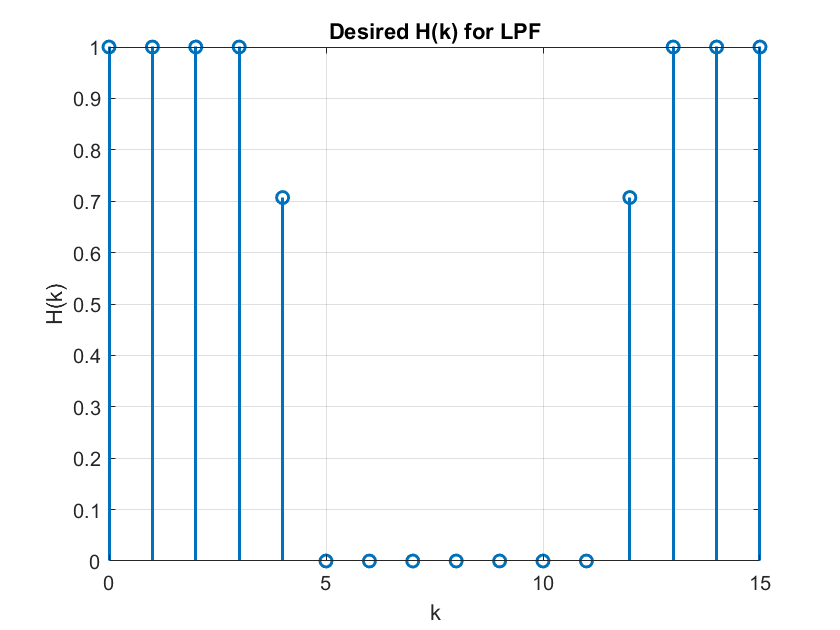
\includegraphics[width=0.5\textwidth]{prob1a_array_H.png}}}
				\caption{Plot of the Values in the Array \texttt{H}}
			\end{figure}
			
			\item Compute the inverse DFT using \texttt{h = ifft(H)}. Show the values you obtain. Since $H(e^{j\omega})$ and $H(k)$ are real and even in the equations above, we expect that the imaginary part of the inverse FFT should be approximately zero. Plot the resulting \texttt{h(n)} for \texttt{n = 0} to \texttt{15}. For example, in MATLAB you can do \texttt{n = 0:15; stem(n,h)}.
			
			\begin{figure}[H]
				\centerline{\fbox{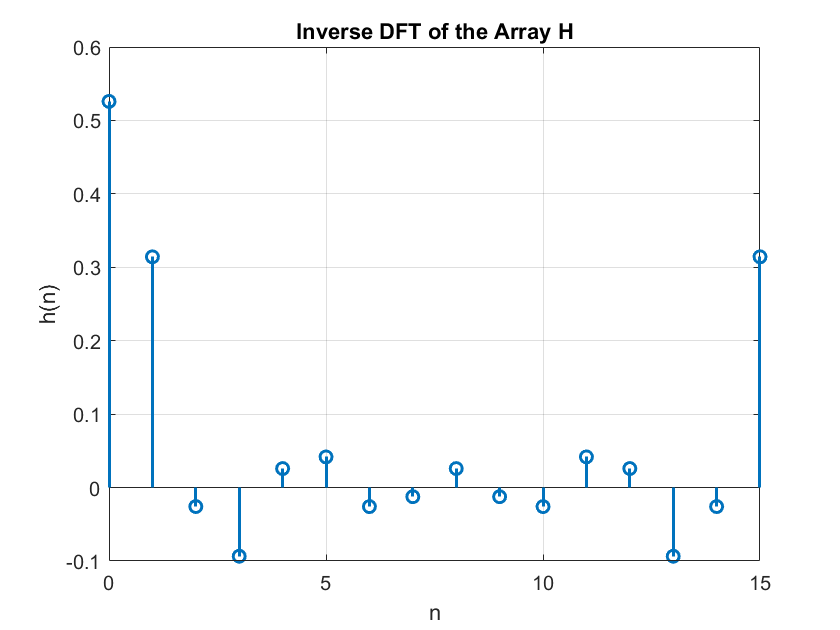
\includegraphics[width=0.5\textwidth]{prob1b_ifft_of_H.png}}}
				\caption{Inverse DFT of the Array \texttt{H}}
			\end{figure}
			
			\pagebreak
			\item Using 16 samples over $0 \leq \omega < 2\pi$, plot the frequency response. For example, in MATLAB:
			
			\texttt{H = fft(h);}
			
			\texttt{stem(abs(H))}
			
			How does this plot compare to the ideal frequency response?
			
			\begin{figure}[H]
				\centerline{\fbox{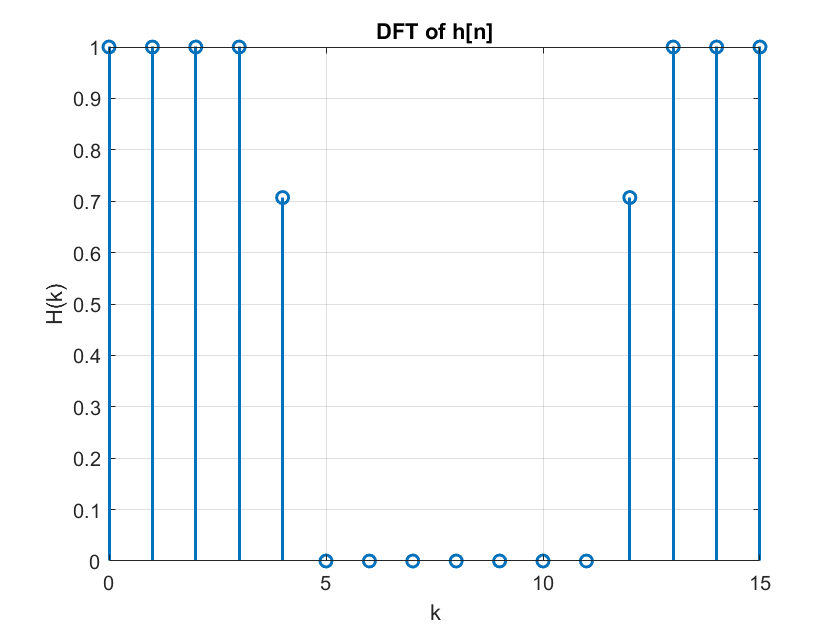
\includegraphics[width=0.5\textwidth]{prob1c_freq_response.png}}}
				\caption{DFT of $h[n]$}
			\end{figure}
			
			Note that the frequency response matches the ideal frequency response exactly at each of the frequencies samples we specified when defining $H(k)$.
			
			\item Rearrange the elements of \texttt{h} to obtain a causal, symmetric impulse response, \texttt{hc}. Plot the result. For example, in MATLAB do \texttt{stem(hc)}. What is the final length of this filter?
			
			\begin{figure}[H]
				\centerline{\fbox{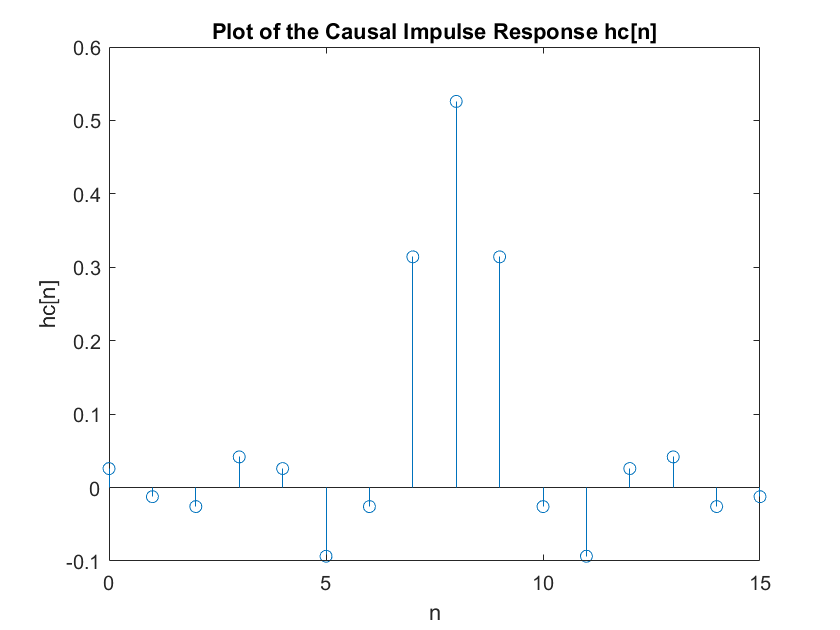
\includegraphics[width=0.5\textwidth]{prob1d_causal_impulse_response.png}}}
				\caption{Causal Impulse Response $hc[n]$}
			\end{figure}
			
			The final length of the symmetric causal filter is 17. The first and last samples are $h[8]/2$. When the filter is turned in a discrete Fourier series with period 16. The first and last samples of the causal filter add together to produce the correct starting sample. 
		\end{enumerate}
	\end{enumerate}
	
	
	
\end{document}